%!TEX root = main.tex

\subsection{Introduction}\label{intro}
Consider a multi-armed bandit problem with $n$ arms where the $j$th pull from the $i$th arm emits an independent random variable $X_{i,j} \in [0,1]$ with $\mu_i:=\E[X_{i,j}]$. 
Given $\epsilon,\delta \in (0,1)$, how many total pulls must an algorithm make in order to return an arm $\widehat{i} \in \{1,\dots,n\}$ with a \emph{small}\footnote{While non-standard in stochastic bandits, seeking small means significantly simplifies notation in the infinite-armed bandit setting; we translate all prior results to this equivalent perspective.} mean that satisfies $\mu_{\widehat{i}} \leq \displaystyle\min_{j} \mu_j + \epsilon$ with probability at least $1-\delta$?
Much effort has gone into answering this and closely related questions resulting in a rich collection of algorithms.
But each algorithm starts the same:  \textit{Pull each arm $i \in \{1,\dots,n\}$ once.}
% \begin{quote}

% \centerline{}
% \end{quote}
%
%
\begin{wrapfigure}{r}{0.45\textwidth}
% \vspace{-2.5em}
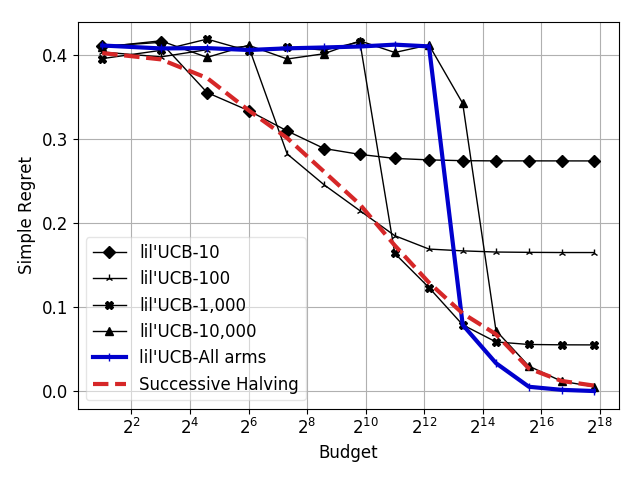
\includegraphics[width=.45\textwidth]{fixedbudget/figures/folder5/new_yorker.png}
\caption{$3,795$ arms. Difference of the recommended and optimal arm's mean as a function of total pulls. }
\label{fig:newyorker}
\vspace{-1.5em}
\end{wrapfigure}
%
%

In this work we are interested in problems where the number of arms $n$ is so large that it is dwarfed by any available budget of total pulls. Furthermore, we make no assumptions about the so-called arm reservoir.
Necessarily, we are interested in problems where the budget necessary to identify an $\epsilon$-good arm among the $n$ arms with probability $1-\delta$ is \emph{independent} of $n$. 
% Ignoring $\log\log$ factors, it is known that $B = O\left( \sum_{i=1}^n \max\{ (\mu_1 - \mu_i)^{-2}, \epsilon^{-2} \} \right)$ total pulls are \emph{sufficient}.
 % which one notes is always $\Omega(n)$ scaling at least linearly with the number of arms $n$. 
% While \emph{sufficient}, we show that this $\Omega(n)$ number of samples may be far from \emph{necessary}, and that in many natural situations $B$ need not have any dependence on $n$!
% Indeed, this work studies the case when $n \gg B$, that is, when the number of arms $n$ far exceeds the allowable total number of pulls $B$.
Such cases arise when the proportion of $\epsilon$-good arms is independent of $n$ (e.g. $\frac{1}{n} \sum_{i=1}^n \1\{ \mu_i \leq \min_j \mu_j + \epsilon\} \geq \epsilon^2$).

Consider a concrete example of the New Yorker caption contest dataset,
where captions are voted on to find the funniest one (see Section~\ref{experiments}).
The bold blue line is the best-arm identification algorithm lil'UCB \citep{Jamieson2014lilU} executed on all $3,795$ arms, lil'UCB-$X$ for $X$ in $\{10,100,1000,10000\}$ is lil'UCB run on $X$ arms randomly drawn with replacement from the $3,795$ arms, and ISHA is the proposed algorithm of this work. Each algorithm outputs the empirical best arm at any given total budget of pulls, breaking ties randomly.
We observe that one can identify a ``pretty good'' arm faster when the number of drawn arms $X$ is small, but as a consequence this small set of arms will not have an arm very close to the best possible arm.
We also observe that ISHA appears to naturally navigate this tradeoff.  

When $n \gg T$ we can treat $n$ as effectively \emph{infinite} and the difference between sampling an arm with or without replacement is indistinguishable. 
Towards this end, we define the \emph{infinite-armed bandit problem}.

\subsubsection{The Pure-exploration Infinite-armed Bandit Problem}
Let $\nu_0$ be a fixed but arbitrary cumulative distribution function over $\R$ such that if $\boldsymbol{\mu} \overset{iid}{\sim} \nu_0$ then $\P(\boldsymbol{\mu} \leq x) = \nu_0(x)$. 
In the finite-armed bandit case like the example of the previous section, one would take $\nu_0(x) = \frac{1}{n} \sum_{i=1}^n \1\{\mu_i \leq x \}$.
Without loss of generality $\{\mu_i\}_{i=1}^\infty$ are drawn i.i.d. from $\nu_0$ before the start of the game and identified by their index, and the player has no prior knowledge of $\nu_0$.
Consider the pure-exploration infinite-armed bandit game.

\begin{figure}
\centering
\fbox{
	\begin{minipage}{.95\textwidth}
	\textbf{Pure-exploration Infinite-armed bandit game}
	\hrule
	\vspace*{.05in}
	\textbf{Input} $\epsilon,\delta \in (0,1)$ and reservoir distribution $\nu_0$\\
	\textbf{Initialize} Draw $\{\mu_i\}_i \overset{iid}{\sim} \nu_0$ 
	    and set $N_i(t) := \sum_{s=1}^t \1\{I_s = i\}$ for all $t \in \mathbb{N}$\\
	\textbf{for} $t=1,2,\dots$\\
	\hspace*{.25in} Player chooses $I_t \in \mathbb{N}$ \\
	\hspace*{.25in} Nature reveals $X_{I_t,N_{I_t}(t)} \in \R$ 
	    where $\E[X_{I_t,N_{I_t}(t)} | I_t ] = \mu_{I_t}$ \\
	\hspace*{.25in} Player recommends $J_t \in \mathbb{N}$
	\end{minipage}
}
\vspace{-.25in}
\end{figure}
% If $Z_t := X_{I_t,N_{I_t}(t)}$ then given the filtration $\mathcal{F}_t = ( (I_1, Z_1, J_1), \dots, (I_t, Z_t, J_t))$ we have that $I_t$ is $\mc{F}_{t-1}$ measurable, $Z_t$ is $\mc{F}_t$ measureable, and $J_t$ is $\mc{F}_t$ measureable.


\noindent\textbf{Goal:} For a fixed reservoir distribution $\nu_0$ with $\mu_* = \inf \{ x : x \in \text{support}(\nu_0) \}$ and $\epsilon \in (0,1)$, how big must $\tau \in \mathbb{N}$ be to ensure that $\mu_{J_\tau} \leq \mu_* + \epsilon$ with high probability?

\noindent Said another way, minimize \emph{simple regret} \citep{bubeck2009pure,DBLP:journals/corr/CarpentierV15} in high probability, which implies a bound on $\E[\mu_{J_t}]-\mu_*$ (see Remark~2).

% An important deviation of this simple regret objective from the fixed confidence setting of PAC-learning for multi-armed bandits \cite{EvenDaral06,DBLP:conf/icml/KalyanakrishnanTAS12,icml2013_karnin13,Jamieson2014lilU} is that in the defined infinite armed-bandit problem \emph{the player never decides to stop and output an arm}.
% Suppose the player \emph{did} stop at some finite time under some distribution $\nu$. 
% Because the player has no knowledge of $\nu$, an adversary could look at the player's algorithm and cook up an alternative distribution $\nu'$ that has a very tiny amount of mass near $-\infty$ such that the player would never observe it and be unable to distinguish $\nu$ versus $\nu'$, stop early, and never output an $\epsilon$-good arm. 
% Such an example precisely explains why \emph{finite-armed bandit lower bounds with stopping times} necessarily scale like $\Omega(n)$ \cite{kaufmann2016complexity,simchowitz2017simulator}: the player must sample each arm a minimum number of times to rule it out as $\epsilon$-good.
% Of course, a sample complexity $\Omega(n)$ is meaningless in the infinite-armed bandit when $n$ is infinity, hence, we focus on simple regret \cite{bubeck2009pure,DBLP:journals/corr/CarpentierV15} versus PAC.

% We stress that there are many related and previous works that address different infinite-armed bandit settings that are reviewed in Section~?.
% However, to the best of our knowledge this particular pure-exploration objective in its full generality (e.g., arbitrary reservoir distribution $\nu$) is novel.  



\subsubsection{Prior work}\label{prior_work}

The main objective of this work is \emph{pure-exploration} where different arms are sampled different numbers of times with the goal of choosing $J_t$ after $t=T$ rounds such that the \emph{simple regret} $\mu_{J_t}-\mu_* \leq \epsilon$ for as small $\epsilon$ as possible. 
Contrast this with \emph{exploration-vs-exploitation} where the objective is to pull different arms to minimize the \emph{cumulative regret} of all the plays of the arms pulled: $\sum_{s=1}^t \mu_{I_s} - \mu_*$.
In pure-exploration the player is only evaluated on the mean $\mu_{J_t}$ of the recommended arm at time $t$; in exploration-vs-exploitation the player is evaluated on all the arms played $\{ \mu_{I_s} \}_{s=1}^t$ up to time $t$. 
The infinite-armed case has also been studied in both the explore-vs-exploit and pure-exploration settings, which we briefly review. 

% Within the pure-exploration literature, two studies have been the focus of study: the \emph{fixed budget} and \emph{fixed-confidence} settings. 
% In the fixed budget setting, given a fixed number of arm pulls the objective is to
% either minimize the simple regret (defined above) or the probability of the strategy not returning the best arm.  In the fixed-confidence setting, the objective is
% to find the best arm W.H.P. using as few total arm-pulls as possible.
% The present work is in the fixed budget pure exploration setting where the number of arms is  infinite.
% To provide context, we will next review the literature in the aforementioned settings.

\paragraph{Explore-vs-Exploit: Minimizing cumulative regret.} 

While research on the finite-armed bandit problem for explore-vs-exploit is quite mature \citep{bubeck2012regret}, many open problems still remain for the infinite-armed setting.
To the best of our knowledge, a form of the infinite armed bandit problem was first proposed in \citet{berry1997} which studies the particular case when observations are Bernoulli and $\nu_0$ is the uniform distribution over a known interval $[a,b] \subseteq [0,1]$, but also considers asymptotic upper bounds for their novel algorithm for a more general class of distributions $\nu_0$. 
This work inspired a number of followup works including \cite{teytaud2007anytime} that extended the algorithm of \cite{berry1997} to settings where the time horizon of the algorithm was unknown in advance.  
These algorithms worked on the principle of flipping a coin until $m$ failures are observed at which time it would discard the current coin and sample a new one from $\nu_0$. 
\cite{bonald2013two} studied a related algorithm for Bernoulli observations where $\nu_0$ is a beta distribution:
\begin{align}\label{eqn:beta_distribution}
\nu(\mu) = \int_{\theta=0}^\mu \tfrac{\Gamma(\alpha_1+\alpha_2)}{\Gamma(\alpha_1) \Gamma(\alpha_2)} \theta^{\alpha_1-1}(1-\theta)^{\alpha_2-1} d\theta
\end{align}
with known parameters $\alpha_1,\alpha_2$; lower bounds are proven for any algorithm in this setting.
Note that \eqref{eqn:beta_distribution} with $\alpha_1=\alpha_2=1$ is just the uniform distribution.

While these previous algorithms assumed that $\nu_0$ was equal to some known parameterization of a beta distribution on a known support, \cite{wang2008} relaxed these conditions to simply assume there exists (known) constants $c,C,\beta,\epsilon_0$ such that 
\begin{align} \label{eqn:beta_parameterization}
c \epsilon^\beta \leq \nu_0(\mu_* + \epsilon) \leq C \epsilon^\beta \qquad \forall \epsilon \leq \epsilon_0.
\end{align}
Clearly, for sufficiently small $\epsilon_0$ the beta distribution of \eqref{eqn:beta_distribution} satisfies \eqref{eqn:beta_parameterization} with $\mu_*=0$ and $\beta = \alpha_1$.
In this more general setting \cite{wang2008} proposed an algorithm with cumulative regret guarantees that only needed to know $\beta$, not the support or $\mu_*$.
\citet{Chan2018Infinite} recently proved lower bounds and proposed an algorithm based on confidence intervals.
% And \cite{li2017infinitely} studied another variant under \eqref{eqn:beta_parameterization} where arms have different costs to pull.
To our knowledge, there exists no algorithm in the regret setting that provably adapts to general, unknown reservoir distributions $\nu_0$ with near-optimal cumulative regret. 

A related problem is when each arm's reward distribution is a single-point distribution, or deterministic, but unknown until it is played.
In this setting \cite{david2014infinitely,david2015refined} studied reservoir distributions with conditions similar to \eqref{eqn:beta_parameterization}.

Quantiles are a convenient object in infinite armed bandits since one can very accurately determine how many arms must be sampled to obtain at least one in the $q$th quantile without knowing anything about $\nu_0$. 
% Contrast this with our setting where it is impossible a priori without knowledge of $\nu_0$ to know how many arms must be sampled to obtain one within $\epsilon$ of $\mu_*$. 
In the quantile-regret minimization setting where $\mu_q$ denotes the $q$th percentile of $\nu_0$ for any $q \in (0,1)$, \cite{chaudhuriquantile} provide an algorithm that obtains sub-linear regret with respect to $\mu_q$ (instead of $\mu_*$) for arbitrary reservoir distributions $\nu_0$.

\paragraph{Pure exploration: Simple regret, fixed budget, fixed confidence.}
% Similarly, the finite-armed pure-exploration setting is quite mature and has been studied under a number of metrics which we briefly review. 
% \citet{bubeck2009pure} studied algorithms and limits on the behavior of \emph{simple regret} $\mu_{J_t}-\mu_*$ as a function of $t$. 
% In the \emph{fixed budget} setting \cite{audibert2010best}, the algorithm takes a budget $B$ as input and outputs a single arm $\widehat{i} \in [n]$ and the algorithm is evaluated based on the rate at which $\P( \widehat{i}_B \neq \min_j \mu_j)$ decreases to zero as a function of $B$. 
% The Successive Halving algorithm for the fixed budget setting was proposed in \cite{icml2013_karnin13} which the current work borrows for its algorithm with a particular parameterization.
% One notes that one can trivially obtain simple-regret guarantees from a fixed-budget algorithm.
% Lower bounds were proved for the fixed budget setting in \cite{carpentier2016tight}.
% Finally, in the \emph{fixed confidence (or PAC)} setting the algorithm takes $\delta,\epsilon>0$ as input and attempts to minimize the number of samples before outputting an arm within $\epsilon$ of the best possible with probability at least $1-\delta$ \cite{EvenDaral06, DBLP:conf/icml/KalyanakrishnanTAS12,NIPS2012_4640, icml2013_karnin13,Jamieson2014lilU}. Lower bounds on the sample complexity for this finite bandit problem are also known \cite{Mannor04thesample,kaufmann2016complexity}. 


The infinite-armed bandit setting for pure-exploration is also well-studied. 
The most-biased coin problem is a particular instance where 
\begin{align}\label{eqn:mostbiasedcoin_reservoir}
\nu_0(\mu) = \int_{\theta=0}^\mu \pi \delta_{\rho}(\theta) + (1-\pi) \delta_{\rho+\epsilon}(\theta) \, d\theta
\end{align} 
where $\delta_{x}(\theta)$ is a Dirac-delta at $x$ and parameters $\rho,\pi,\epsilon \in (0,1)$ are known \citep{chandrasekaran2014finding,malloy2012quickest} and unknown \citep{jamieson2016power}.
This parameterization is thought to be difficult because there is no incremental improvement towards the optimal arm over time: the optimal arm has either been identified or it has not. 
 % knowledge of the means of sub-optimal arms provides no knowledge about the value of the optimal mean in the sense that \eqref{eqn:beta_parameterization} does by being able to extrapolate\footnote{This property was used by \cite{DBLP:journals/corr/CarpentierV15} to adapt to unknown $\beta$ in the model of \eqref{eqn:beta_parameterization}.}.
Quantile problems have also been studied in the pure-exploration setting, such as identifying an arm $\epsilon$-close to $\mu_q$ \citep{chaudhuri2017pac,aziz2018pure,ren2018exploring}.



% However, in this setting one finds algorithms that are more robust to uncertainty in the form of reservoir distribution $\nu_0$.
\citet{DBLP:journals/corr/CarpentierV15} proposed an algorithm 
known as SIRI
specifically for  reservoir distributions parameterized as \eqref{eqn:beta_parameterization}.
Remarkably, they show that they can adapt to unknown parameters of this parametric model achieving a simple regret guarantee of  $r_t=\mathcal{O}\left( \max\left(t^{-1/2}, t^{-1/\beta}\polylog(t)\right)\right)$ with high probability for their algorithm; they also provide nearly-matching lower bounds on simpler regret for the $\beta$-parameterization of \eqref{eqn:beta_parameterization}.
\citet{li2017hyperband} proposed the Hyperband algorithm which, to our knowledge, is the only algorithm to obtain simple regret guarantees for general, unknown reservoir distributions (i.e., without a known parameterization like \eqref{eqn:beta_distribution}-\eqref{eqn:mostbiasedcoin_reservoir} of any kind).
For any $\epsilon>0$ and reservoir distribution $\nu_0$, they show that the simple regret of Hyperband is bounded by $\epsilon$ with high probability once the budget $t$ exceeds 
\begin{align}\label{eqn:rough_sample_complexity}
\epsilon^{-2} + \tfrac{1}{\nu_0(\mu_* + \epsilon)}\int_{\mu_*+\epsilon}^\infty \tfrac{1}{(\mu-\mu_*)^2} d\nu_0(\mu)
\end{align}
pulls (up to poly-logarithmic factors).
This result matches all known pure-exploration upper bounds, even those algorithms designed for specific reservoir distributions, up to poly-logarithmic factors.
For any given value of $n \in \mathbb{N}$, Hyperband is nothing more than running $\log_2(n)$ copies of the Successive Halving algorithm of \cite{icml2013_karnin13} each with a budget of $n$ and $2^k$ arms drawn from $\nu_0$ for $k=1,2,\dots,\log_2(n)$; the whole procedure uses $n \log_2(n)$ total samples. 
While Hyperband is state-of-the-art, hedging over these $\log_2(n)$ copies of Successive Halving is inelegant, and empirically it was almost always observed that the most aggressive bracket with the most arms worked best. 


\subsubsection{Main Contributions}
In this work we show that running just one version of Successive Halving, named ISHA, with $n$ arms and a budget of $n\log_2(n)$ pulls--where arms start being discarded after being pulled just once--achieves better simple regret performance than the state-of-the-art Hyperband, but the algorithm is considerably simpler.

We further show that our proposed algorithm is not only superior on most reservoir distributions (including those derived from finite-armed problems) but also against algorithms that were designed specifically for the reservoirs we evaluated them on, like parameterizations \eqref{eqn:beta_distribution}-\eqref{eqn:mostbiasedcoin_reservoir}.

We conjecture that for any reservoir distribution $\nu_0$ and $\epsilon,\delta$, and for sufficiently large $n$ this procedure returns an $\epsilon$-good arm with probability at least $1-\delta$.

Our second contribution is an information theoretic \emph{lower bound} for the infinite-armed bandit problem. 
Specifically, for any reservoir distribution $\nu$ and any fixed $\epsilon,\delta \in (0,1)$ we prove a lower bound on the expected number of samples any algorithm must make in order to identify an $\epsilon$-good arm with probability at least $1-\delta$ that depends on $\nu,\epsilon,\delta$. 
The conjectured upper bound and the lower bound match the expression of \eqref{eqn:rough_sample_complexity} up to possible logarithmic factors.  


